\chapter{Evaluation}
\label{ch:eval}


\section{Comparison with \porthos[1]}
\label{ch:eval:show}

Consider two equivalent functions \texttt{t0} in Figure~\ref{ex:test-both-cf}: in the C language (left) and in the \porthos[1] input language (right).
The functions contain three nested \texttt{while}-loops and thus can serve as an illustration of differences in the program compilation and unrolling processes between \porthos[1] and \porthos[2].

\begin{figure}[!h]
\begin{subfigure}[b]{.53\textwidth}\centering
\begin{lstlisting}[language=Java,basicstyle=\ttfamily\small]

void t0(int &x) {
     int a = 1;
     int c = 1;
     while (a == 1) {
         int b = 1;
         while (b == 1) {
             while (c == 1) {
                 x = c;
             }
             x = b;
         }
     }
     x = a;
 }
 
 
\end{lstlisting}
\caption{An example in the C language}
\label{ex:both-cf:ptsC}
\end{subfigure}
\begin{subfigure}[b]{.45\textwidth}\centering
\begin{lstlisting}[language=Java,basicstyle=\ttfamily\small]
{ x }
thread t0 {
     a <- 1;
     c <- 1;
     while (a == 1) {
         b <- 1;
         while (b == 1) {
             while (c == 1) {
                 x := c
             };
             x := b
         };
     };
     x := a
 }
\end{lstlisting}
\caption{An example in the \porthos[1] input language}
\label{ex:both-cf:pts1}
\end{subfigure}
\caption{Example: A demonstrative cyclic function}
\label{ex:test-both-cf}
\end{figure}

The functions are analysed for reachability of the final state by \porthos[2] and modified version \porthos[1] which is able to render the program AST to an event-based control-flow graph (for that, the branching statement \texttt{if-then-else}, the \texttt{while} loop and the \texttt{sequence} statement are expanded recursively and the head and the tails of each instruction are bound by the method processing the parent).
The graph generation is performed via the open-source library \texttt{Graphviz}~\cite{ellson2001graphviz}).
%Each event of the control-flow graph contains the unique number (generated by the \texttt{hashCode} method) in curly brackets below the value, which is necessary for correct displaying the graph.


\subsection{Compilation}
\label{ch:eval:show:compil}

Figure~\ref{ex:test-both-pic} illustrates the data structure which the functions in Figure~\ref{ex:test-both-cf} are compiled to.
The left-hand side picture represents the non-unrolled \xgraph[CF] generated by \porthos[2], and the right-hand picture represents the AST generated by \porthos[1].

In both pictures, the writes are denoted with the left-directed arrow `\lstinline{<-}', and the functions \lstinline{load} and \lstinline{store} denote the type of the shared memory event.
The primary transitions that denote unconditional jumps or if-true-transitions are pictured with solid lines, and the alternative transitions that denote if-false-transitions are pictured with dotted lines.
The graphs contain a single source event and a single sink event represented by the dark-grey triangles (in fact, the graph produced by \porthos[1] does not have sink and source nodes, but they were added to the picture for demonstrative purposes).
For clarity, all branching events, that in current example serve as the conditional events of loops, are highlighed with light-grey colour.

\begin{figure}[!h]
%
\begin{subfigure}[b]{.49\textwidth}\centering
  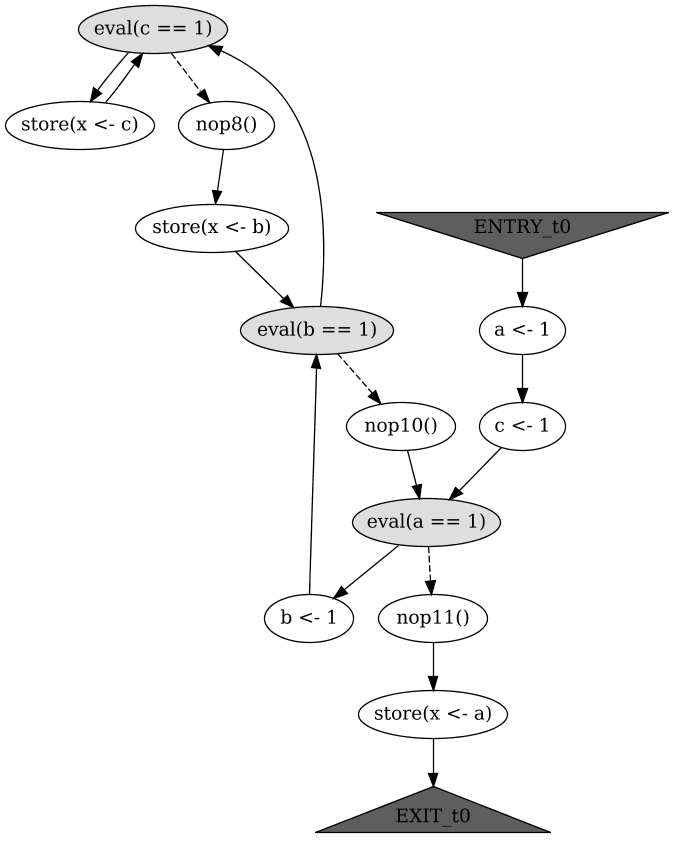
\includegraphics[width=\textwidth,keepaspectratio]{img/my/graphs/unrolling-comparison/PorthosC/t0.png}
  \caption{The compiled \xgraph{} of the function in Figure~\ref{ex:both-cf:ptsC}}
  \label{ex:both-cf:graph:ptsC}
\end{subfigure}
%
\begin{subfigure}[b]{.49\textwidth}\centering	
  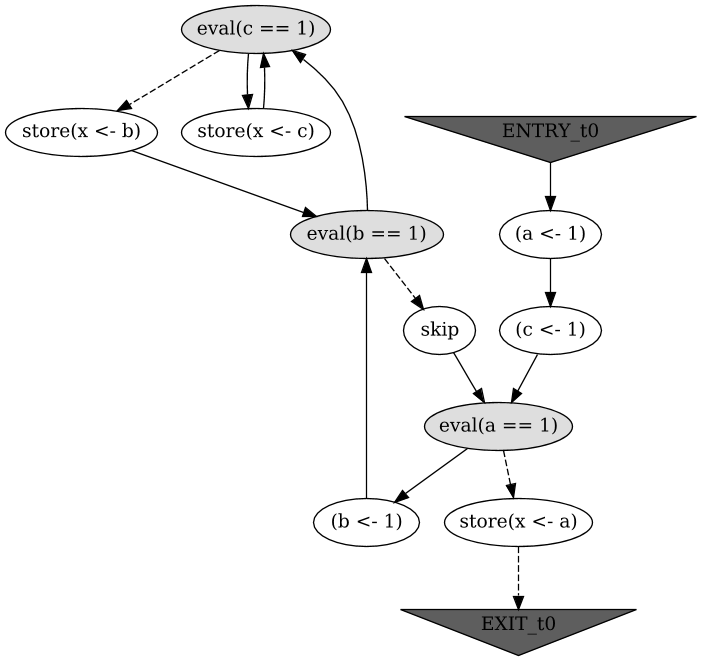
\includegraphics[width=\textwidth,keepaspectratio]{img/my/graphs/unrolling-comparison/Porthos/t0.png}
  \caption{The compiled AST of the function in Figure~\ref{ex:both-cf:pts1}}
  \label{ex:both-cf:graph:pts1}
\end{subfigure}
%
\caption{The control-flow graphs of the functions represented in Figure~\ref{ex:test-both-cf}}
\label{ex:test-both-pic}
\end{figure}

Note that two compiled graphs are equivalent up to the extra \texttt{nop}-events in the \porthos[2] graph, that are necessary for correct encoding as it was discussed in Section~\ref{ch:enc:bmc:cf}, and \texttt{skip}-events in \porthos[1] graph.
However, the unrolled graphs presented in Figure~\ref{ex:test-both-pic-unroll} are different as the tools use different unrolling algorithms.
The labels of events in the left-hand side picture (produced by \porthos[2]) are augmented by the unrolling depth number, which is separated from the event label by comma.


\subsection{Unrolling}
\label{ch:eval:show:unrol}

The unrolling algorithm used by \porthos[1] (right-hand side picture) unrolls \textit{all} loops $k$ times (where $k$ is the unrolling bound), and the unrolling algorithm of \porthos[2] unrolls loops so that not more than $k$ events are executed.
As it is illustrated by the picture, the new algorithm produces a better set of program executions (for example, the unrolled graph of \porthos[1] does not contain executions of the inner loops more than $k=2$ times in a raw, which makes the old unrolling algorithm not complete).
As the new unrolling algorithm is based on the DFS algorithm, it discovers \textit{all} possible paths, therefore the result graph contains \textit{all} possible executions and thus the program analysis performed on this graph can be complete up to bound~$k$.

Note that the unrolled graph produced by \porthos[2] does not necessarily become a tree after removing the sink node.
Some branches of the graph are merged when the executions have the same event with the same unrolling depth number.
For example, primary transitions of both events `\lstinline{[b <- 1, 8]}' and `\lstinline{[store(x <- b), 8]}' (produced by executions of the first iteration of the \texttt{while} loop) lead to the same event `\lstinline{[eval(b == 1), 9]}' (the first event of the second iteration of the second loop).

\begin{figure}%[!h]
%
\begin{subfigure}[b]{.6\textwidth}\centering
  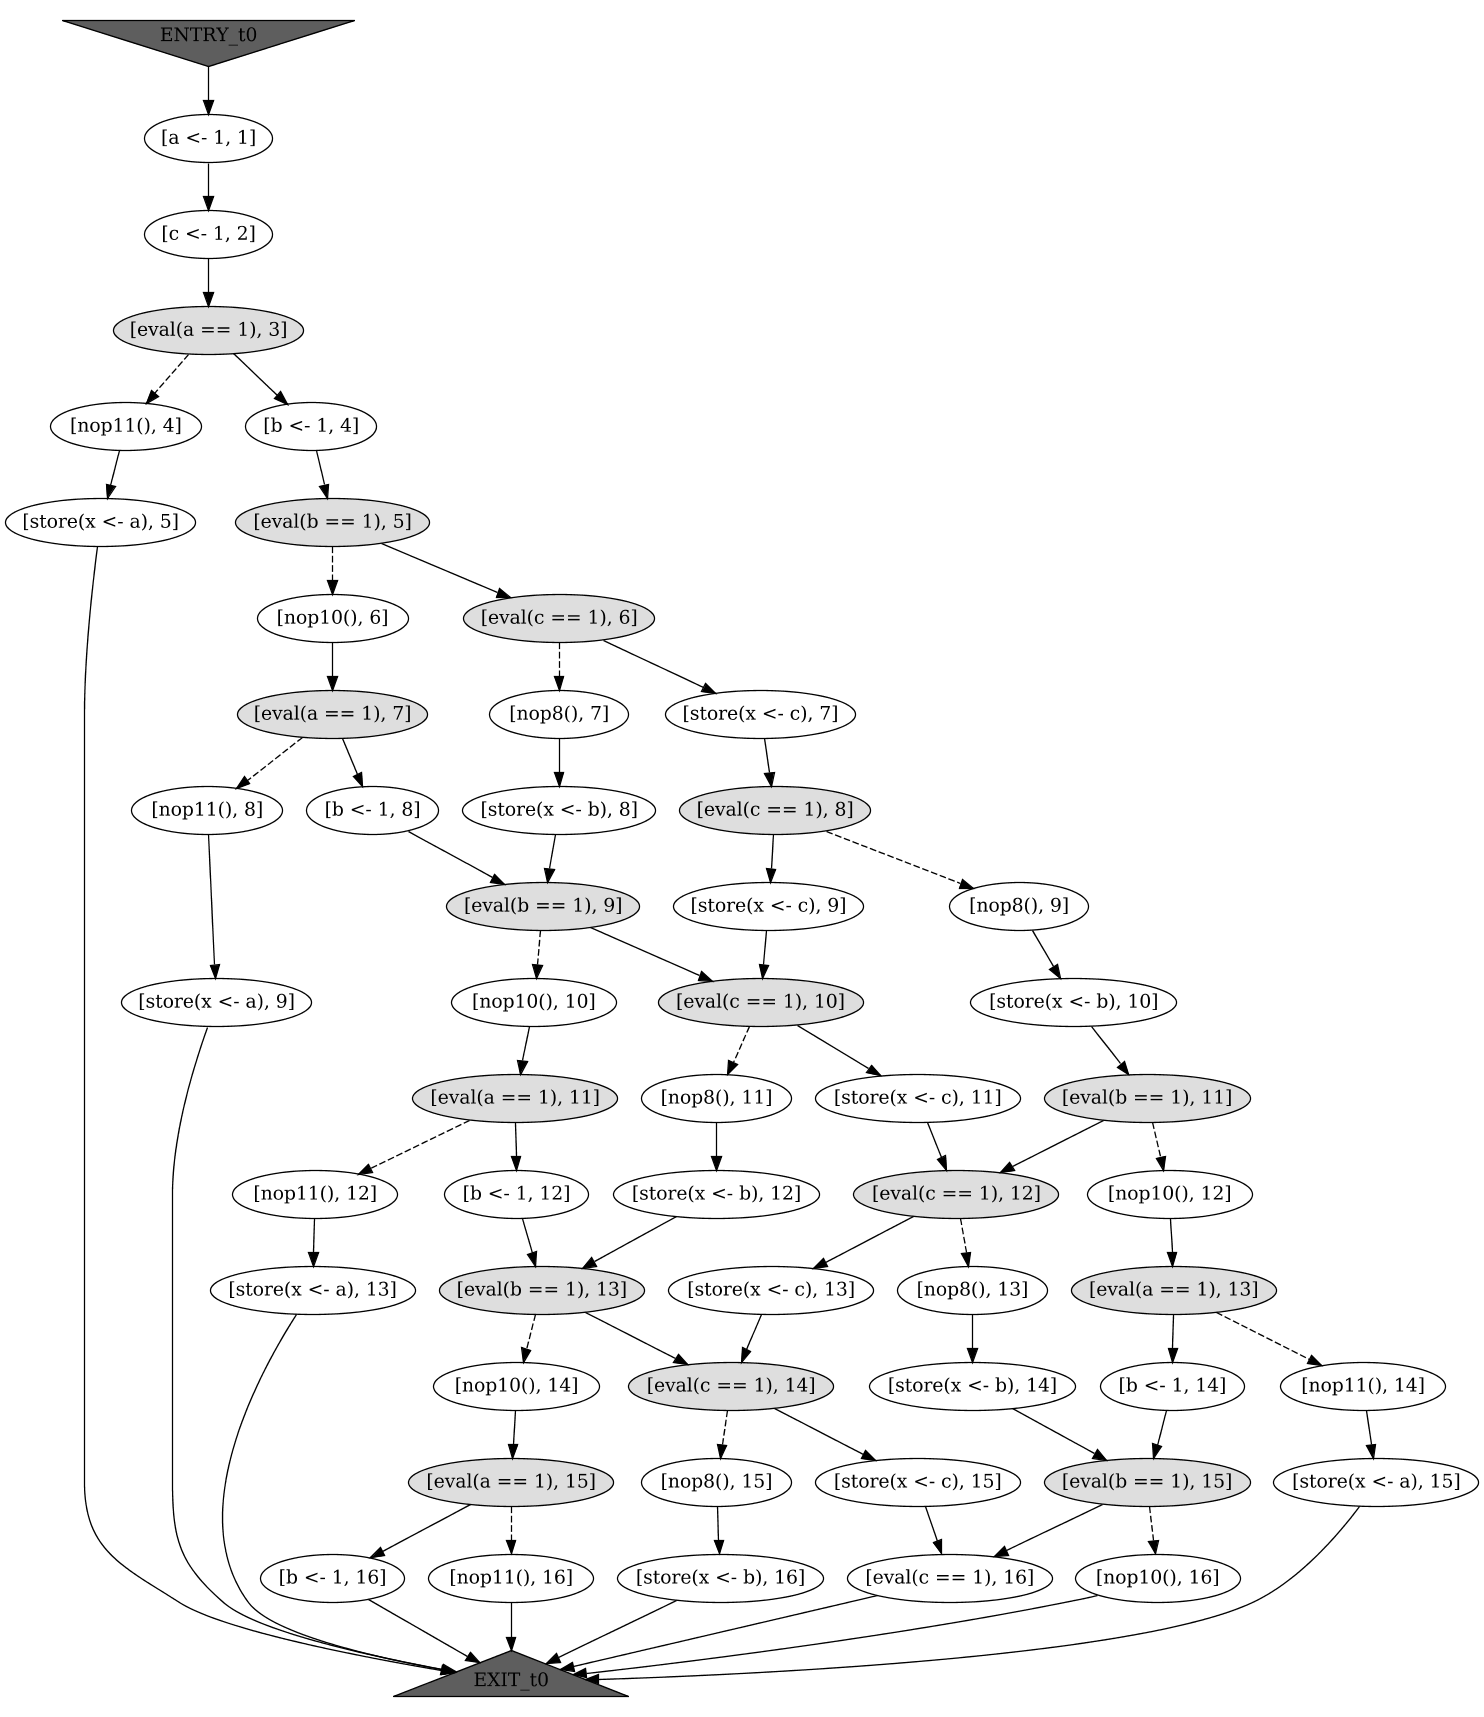
\includegraphics[height=.65\textheight,width=1.1\textwidth]{img/my/graphs/unrolling-comparison/PorthosC/t0_unrolled.png}
  \hfill
  \caption{The unrolled \xgraph{} of the function in Figure~\ref{ex:both-cf:ptsC}}
  \label{ex:both-cf:graphU:ptsC}
\end{subfigure}
\hfill
%
\begin{subfigure}[b]{.3\textwidth}\centering
  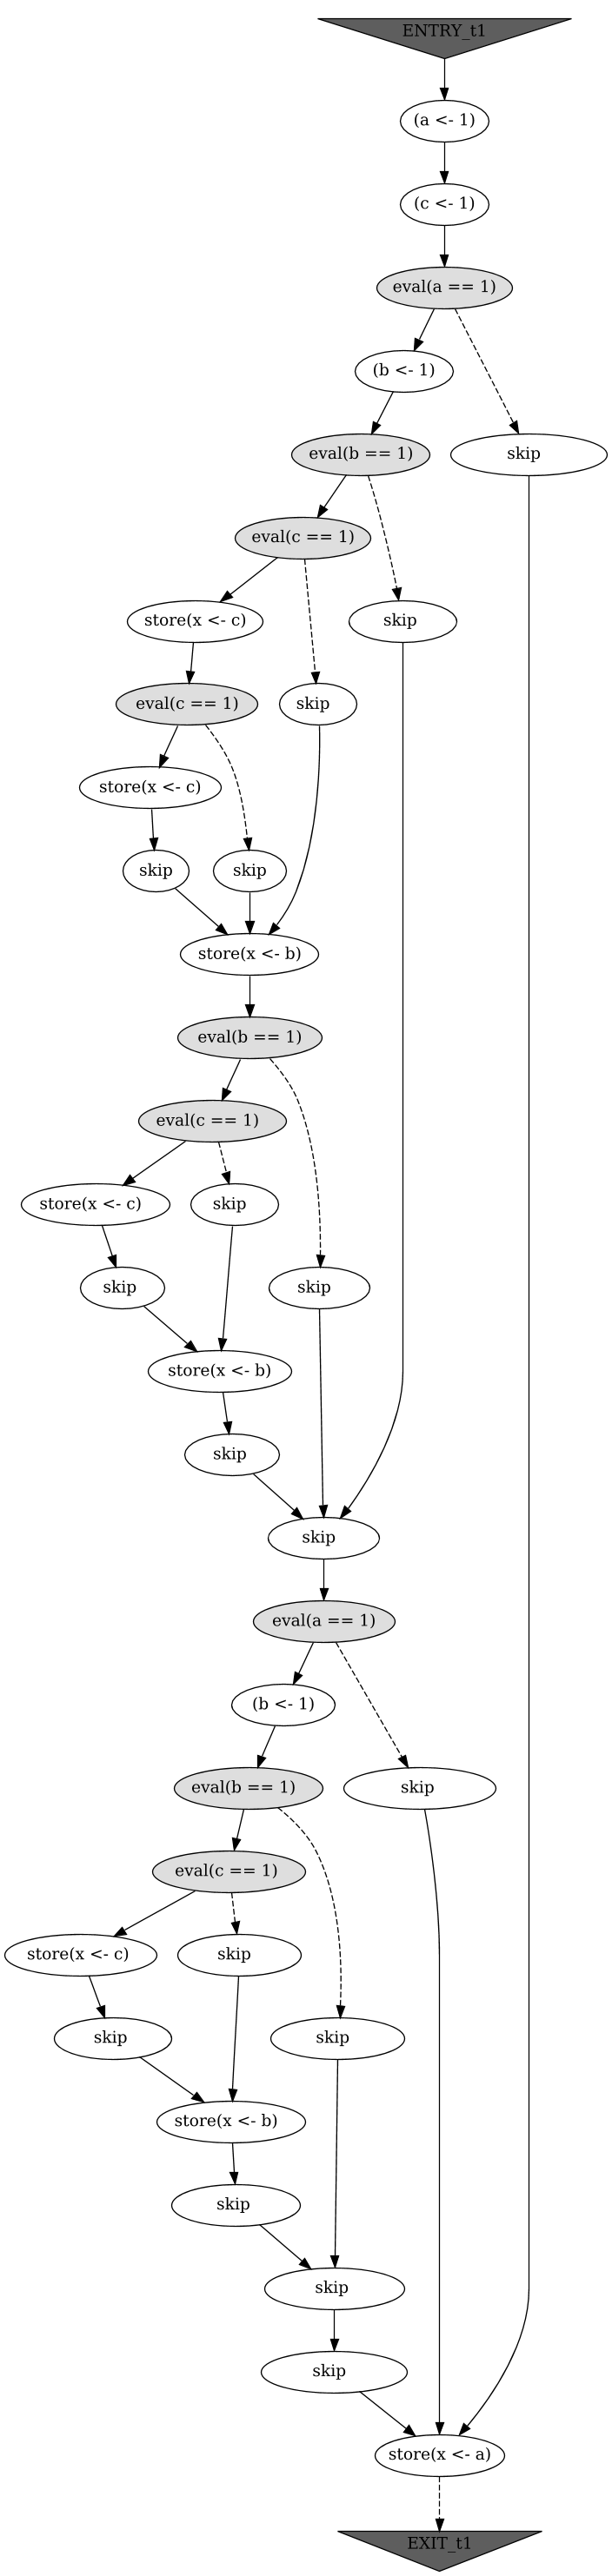
\includegraphics[height=.9\textheight,width=\textwidth]{img/my/graphs/unrolling-comparison/Porthos/t0_unrolled.png}
    \caption{The unrolled AST of the function in Figure~\ref{ex:both-cf:pts1}}
    \hfill
  \label{ex:both-cf:graphU:pts1}
\end{subfigure}
\hfill
%
\caption{The unrolled control-flow graphs of the functions represented in Figure~\ref{ex:test-both-cf}}
\label{ex:test-both-pic-unroll}
\end{figure}

% ---------------------------

\begin{figure}[t]
\begin{subfigure}{.45\textwidth}
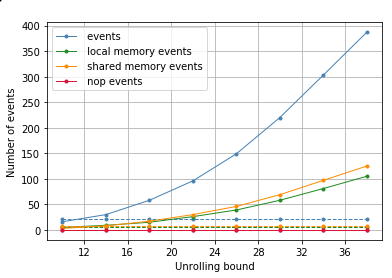
\includegraphics[width=\textwidth,keepaspectratio]{img/my/performance/new/new-e.png}
\caption{The graph unrolled by \porthos[2]}
\label{dep:events:new}
\end{subfigure}
\hfill
%
\begin{subfigure}{.45\textwidth}
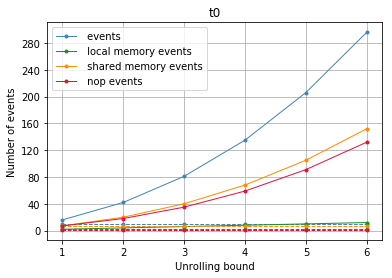
\includegraphics[width=\textwidth,keepaspectratio]{img/my/performance/new/old-e.png}
\caption{The graph unrolled by \porthos[1]}
\label{dep:events:old}
\end{subfigure}
%
\caption{Dependency of number of events in the unrolled Dekker's algorithm on the unrolling bound}
\label{dep:events}
\end{figure}


As another example of program liable for analysis consider the Dekker's algorithm for mutual exclusion of two processes, originally described by Dijkstra~\cite{dijkstra1962over}; the program is presented in Appendix~\ref{apx:dekker}.
For testing \porthos[1], we used the same file in old \porthos{} input language (\texttt{dekker.pts}), which was used in evaluation tests in the original paper~\cite{Porthos17a}.
For performing tests, \porthos[2] was slightly modified in the branch \textit{ay/test-timing}%
\myfootnote{The modifications were pushed into the \porthos[1] repository \url{github.com/hernanponcedeleon/Dat3M}} %
%
for printing detailed timing information and statistics about number of events (commit f8a6c97f) and writing this information in strict \textit{json} format so that it can be easily processed later by a script that analyses and prints the results (commit 48ba7161).
The version of \porthos[2] used for the tests is actual up to commit 01dde6b1 of the \porthos[2] GitHub repository.
Both \porthos[1] and \porthos[2] are run in the state reachability mode for TSO memory model (see sample output of \porthos[2] in Appendix~\ref{apx:output}).

Figure~\ref{dep:events} illustrates the dependency of overall number of events in all unrolled event-flow graphs of the thread \texttt{t0} on the unrolling bound $k$ for the \texttt{Dekker} test (the left-hand side picture illustrates the case for \porthos[2], and the right-hand side picture illustrates the case for \porthos{}).
The solid lines denote dependency of number of unrolled events on the unrolling bound, when the dashed lines denote the number of events in non-unrolled graphs.
%Both charts have limits above $420$ events.
%\porthos[2] (left-hand chart) reaches this limit with the bound $k_2=32$, and \porthos[1] (right-hand chart) reaches it with $k_1=5$.
%However, taking into account the fact that initially both non-unrolled graphs had $20$ events, \porthos[2] at the step $32$ (the longest execution) obtained same number of events  as \porthos[1] at the step $20*5=100$, which shows that it has lost approx. $70$ states.
The blue line depicts the dynamics of the overall number of events in the graph (including memory events, nop events, etc.).
Initially, the thread \texttt{t0} has 22 events.
As in the unrolling scheme of \porthos[1], each loop is executed exactly $k_1$ times, therefore if $k_1=6$, the loop has been executed at least 6 times by producing around $300$ events.
Nonetheless, in the new unrolling scheme used by \porthos[2], the same number of events is produced by the unrolling bound $k_2=34$, which contains approximately $1.5$ executions of the $22$-event loop.
Therefore, according to rough estimates the new encoding scheme produces $6/1.5=4$ times more events than the older one.

The same dynamics can be seen with shared memory events (yellow lines).
However, the new algorithm produces much more local memory events (green line on the left-hand side picture), which grow exponentially with the unrolling bound, when the number of local memory events produced by the old algorithm (green line in the right-hand side picture) grows relatively slowly.
This can be explained by the need to copy all shared variables to local ones when performing computation over them.
On the other hand, the right-hand side picture reveals exponential-like growth of the number of \texttt{nop}- (or \texttt{skip}-) events, that are necessary for implementing the control-flow as an AST, however constitute a redundant part of the model (in the new unrolling scheme, the number of \texttt{nop}-events remains to be relatively constant).

As the new unrolled graph has all possible executions unlike the older one, by default \porthos[2] uses the new unrolling scheme.
However, in some applications the older unrolling mode may be useful (for example, where the user can use other instruments to prove the limitations on the number of executions of a loop), thus the user should be able to change configure the unrolling algorithm (support for the older algorithm is left to a future work).


%The arguments \lstinline{x} and \lstinline{y} of the function are passed by reference, therefore they are treated as global variables.
%The local variable declaration `\lstinline{int r;}' produces no events (it is processed by the X-graph pre-compiler that invokes the memory manager to create the new local variable \lstinline{r}).
%The first event `\lstinline{load(reg_tmp0 <- x}' loads the value of the global variable \lstinline{x} into the temp register \lstinline{reg_tmp0} in order to satisfy the requirement that all computation must be performed over local variables;
%note that each element of the computational tree `\lstinline{eval(eval(eval(5 + eval(eval(4 / 2) * reg_tmp0)) % 3) == 1)}' is represented by a local memory unit (either \texttt{XComputationEvent} or \texttt{XConstant} or \texttt{XRegister}).
%The node of this computational event in the control-flow graph has two outgoing edges, the primary edge to the `\lstinline{load(reg_tmp1 <- y}', the first event of the then-branch of the while-loop, and the alternative edge to the \lstinline{nop}-event representing the only event of the else-branch.

%As is was discussed in Section~\ref{ch:impl:model:xgraph}, all computation events have no impact to the global state of the concurrent system.
%Therefore, the interpreter does not \textit{emit} computational events, but it \textit{creates} them.
%This means, when the \texttt{Y2XConverterVisitor} processes the expression tree `\lstinline{(5 + 4/2 * x) 3 == 1}', it calls the method \texttt{createComputationEvent} of the interpreter that only creates the computation event and does not change its state.
%However, once the converter meets the global variable \lstinline{x}, it calls the interpreter method \texttt{emitMemoryEvent} to copy its value to a temp register; since it meets the global variables involved to the computation before it ends to process the whole computation expression, the values of all these global variables will be copied to temp registers \textit{before} the computation expression is used by any other event.
%Note that if the computation expression has not been used by any other event (for example, as the constant \lstinline{1} in the following C code: `\lstinline{foo(); 1; bar();}'), it is lost from the model (by the term \textit{use} here we mean that the computation event is evaluated as a guard or assigned to another memory unit).


%\subsection{The X-graph unrolling}
%\label{ch:eval:show:unrol}

%Once the \xgraph[CF] is constructed, it should be unrolled to an acyclic flow-graph (as it was discussed in Section~\ref{ch:impl:proc:x-unroll}).
%The Figure~\ref{ex:unrolling} shows the control-flow subgraph \xgraphU[CF] of the event-flow graph from the previous example (see Figure~\ref{ex:compilation}) unrolled up to bound $k=16$.
%

%Also note that comparing to the unrolling bound description given in Section~\ref{ch:impl:proc:x-unroll}, 
%As the distinction between complete and incomplete sink nodes is not implemented yet, 

%\begin{figure}[!h]
%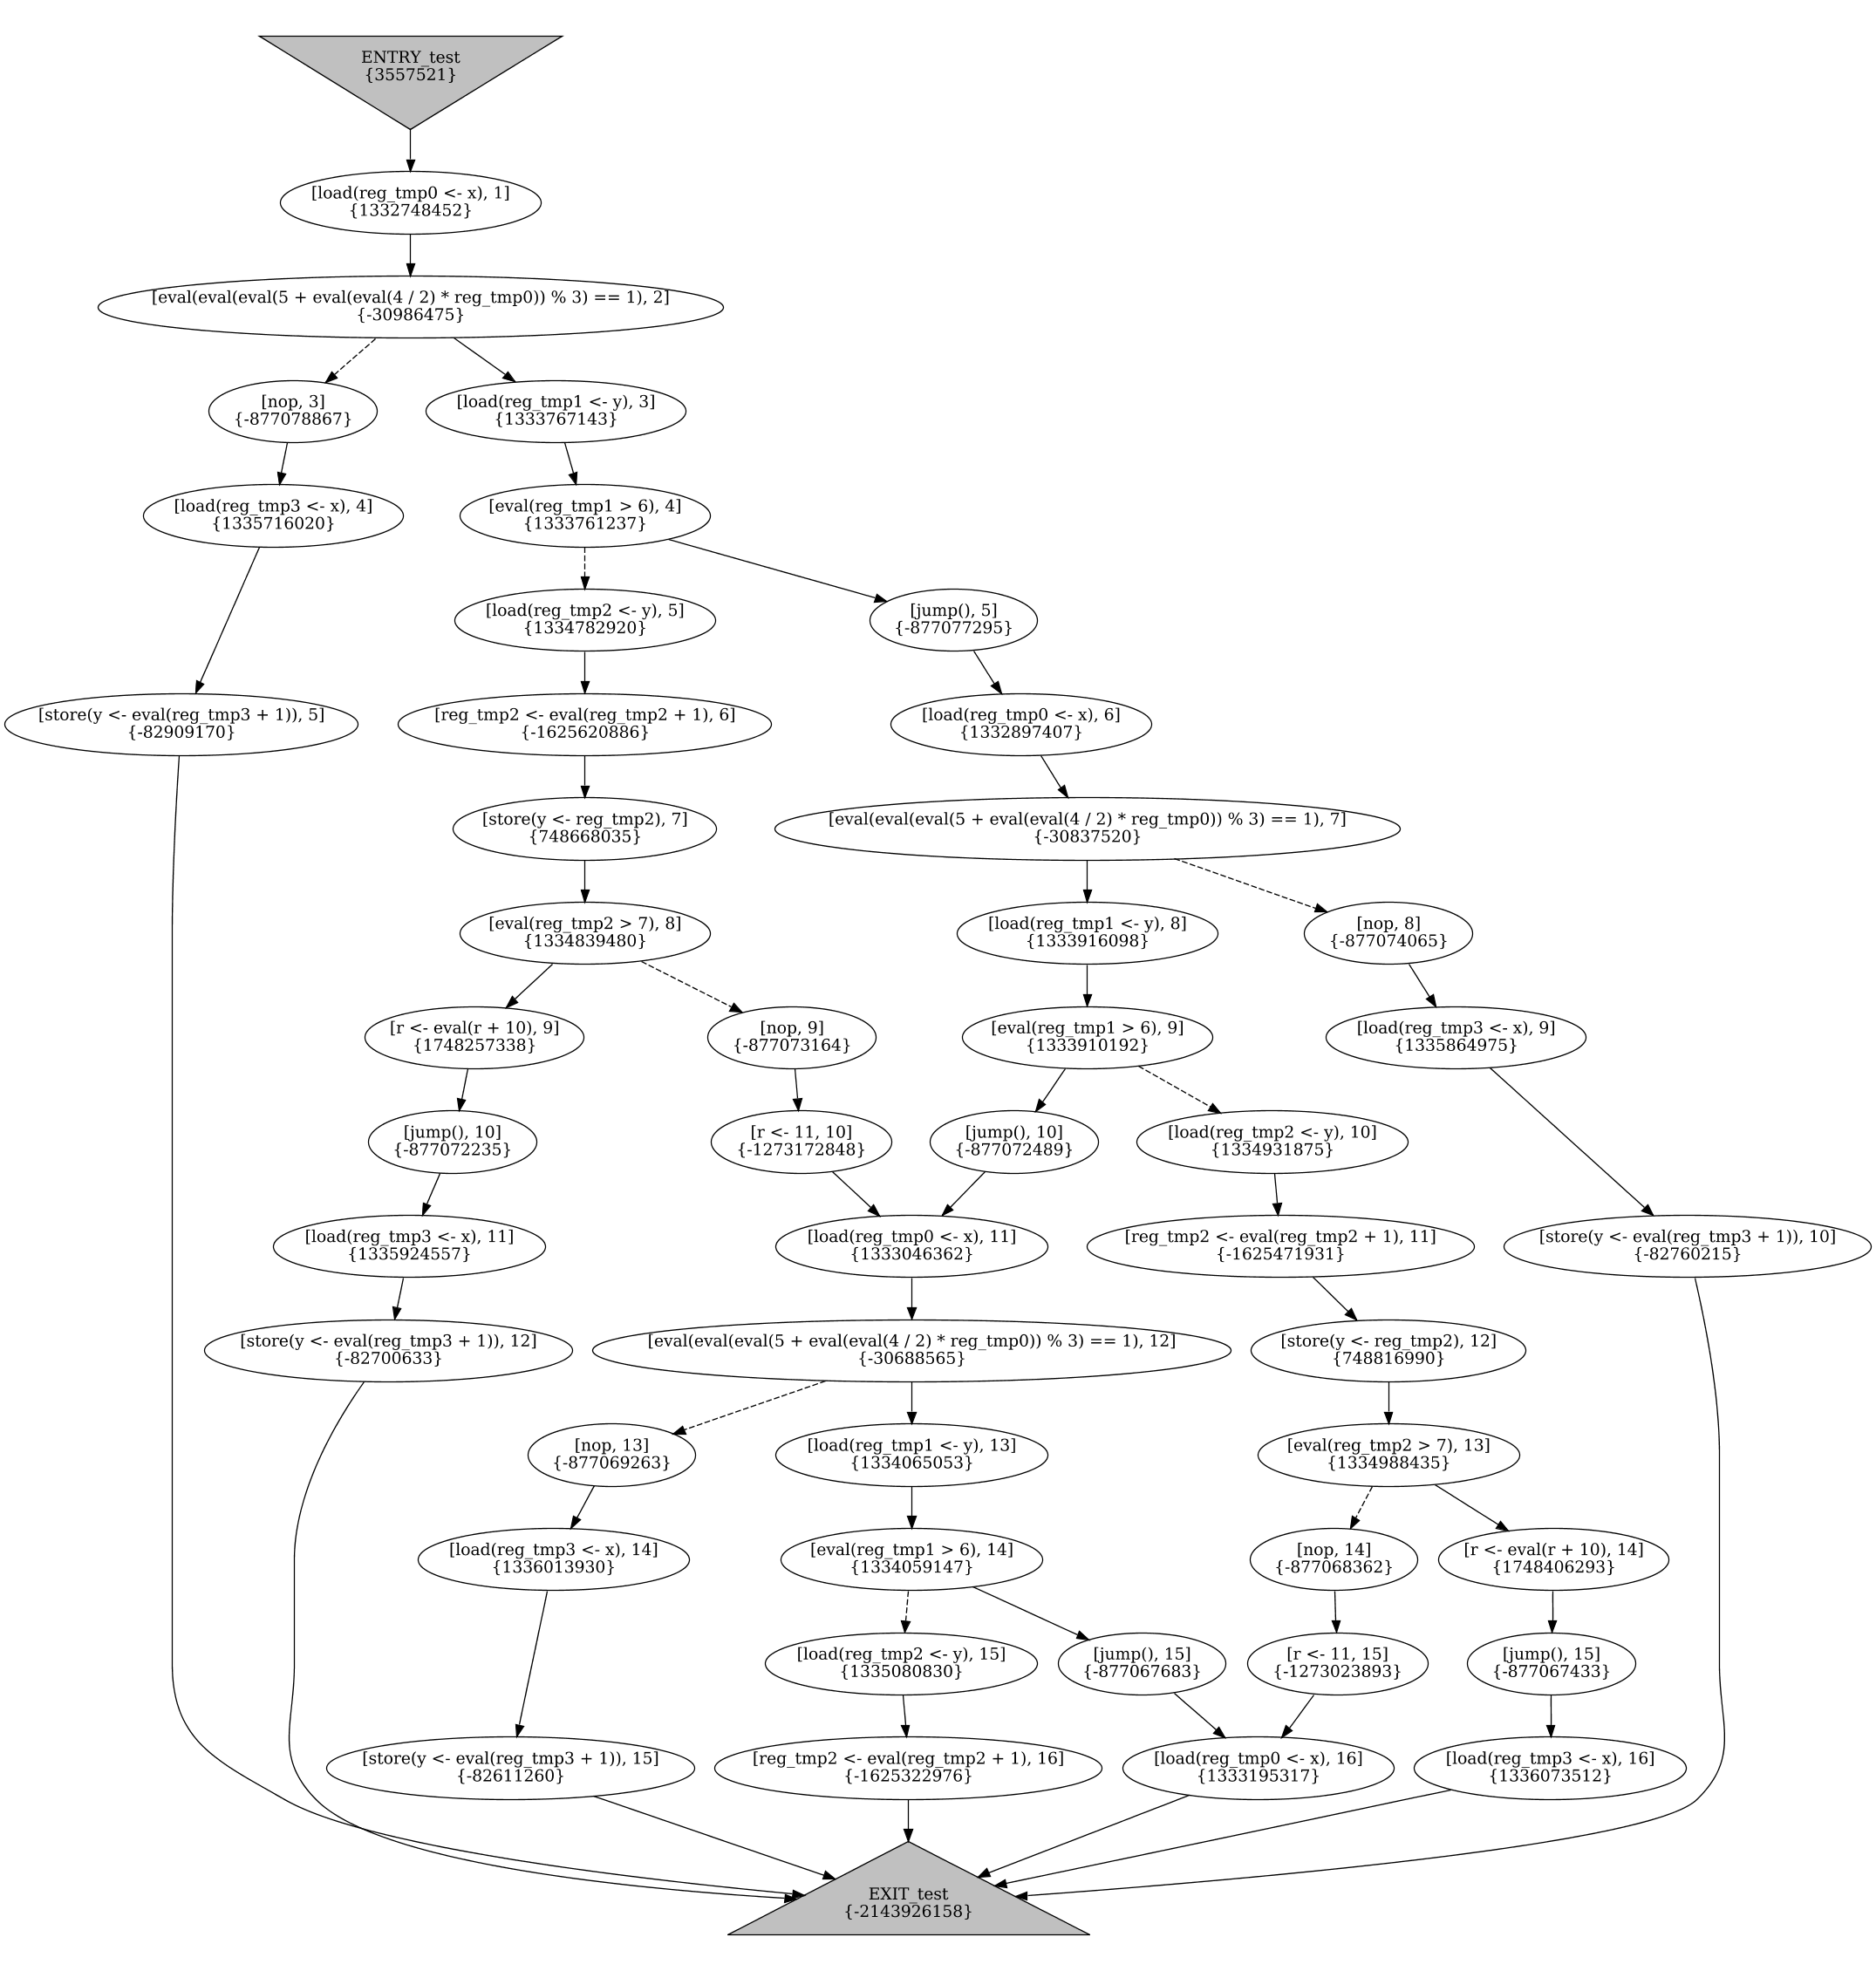
\includegraphics[width=\textwidth,height=\textheight]{img/my/graphs/test_unrolled.png}
%\caption{Unrolling of the event-flow graph presented in Figure~\ref{ex:compilation}}
%\label{ex:unrolling}
%\end{figure}


\section{Performance evaluation}
\label{ch:eval:perf}

Performance evaluation has also been performed on the example of the \texttt{Dekker} test.
%As an example of the C program liable for the reachability and portability analysis, consider the Dekker's algorithm for mutual exclusion of two processes, originally described by Dijkstra~\cite{dijkstra1962over}; the program is presented in Appendix~\ref{apx:dekker}.
%For testing \porthos[1], we used the same file in old \porthos{} input language (\texttt{dekker.pts}), which was used in evaluation tests in the original paper~\cite{Porthos17a}.
For time benchmarking we ran the tools $5$ times and computed the median of the encoding time.
Benchmarking was performed on the Linux machine 8-core Intel(R) Core(TM) i7-3632QM CPU @ 2.20GHz, Java(TM) SE Runtime Environment (build 1.8.0\_161-b12) (Java virtual machine was configured by default parameters).
The time was measured by the tool itself via the native Java method \texttt{System.currentTimeMillis}.

\subsection{State reachability analysis}
\label{ch:eval:perf:reach}

%For checking reachability of the final states of the unrolled graphs compiled for a certain hardware architecture, the tool encodes both program and hardware memory model constraints as it was discussed in Section~\ref{ch:enc:bmc}.
%The result formula is then solved by the Z3 

%TO-DO: fix interface

The sample output of \porthos[2] in the state reachability analysis mode is presented in Appendix~\ref{apx:output}.
The output includes detailed time measurements for each stage of the analysis, and optionally statistical information about the unrolled program (number of events, transitions, etc.)

\begin{figure}[t]
\begin{subfigure}{.45\textwidth}
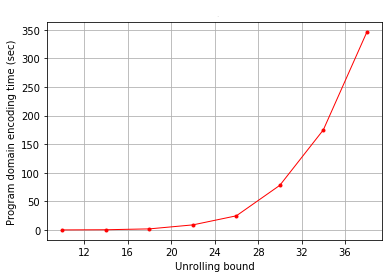
\includegraphics[width=\textwidth,keepaspectratio]{img/my/performance/new/new-t.png}
\caption{Encoding of the graph unrolled by \porthos[2]}
\label{dep:time:new}
\end{subfigure}
\hfill
%
\begin{subfigure}{.45\textwidth}
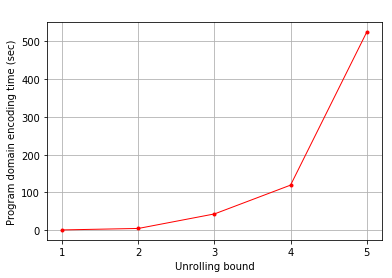
\includegraphics[width=\textwidth,keepaspectratio]{img/my/performance/new/old-t.png}
\caption{Encoding of the graph unrolled by \porthos[1]}
\label{dep:time:old}
\end{subfigure}
%
\caption{Dependency of program domain encoding time (in seconds) on the unrolling bound}
\label{dep:time}
\end{figure}

As the unrolling algorithm has been changed, the number of events after unrolling differs considerably, therefore the correct performance comparison with \porthos[1] is not manageable as the performance of the tools depends directly on number of events.

%For example, with the bound $k_1=2$ \porthos[1] produces $59$ events (among them, $51$ shared-memory events) with the program domain encoding time 4.608 sec,
%and with the bound $k_1=3$ \porthos[1] produces $95$ events (among them, $107$ shared-memory events) with the program domain encoding time 21.475 sec;
%whereas \porthos[2] with the bound $k_2=17$ produces $57$ ($31$) events with the program domain encoding time 1.734, and with the bound $k_2=27$ it produces $193$ events (among them, $107$ shared-memory events, which equal to the number of shared-memory events produced by \porthos[1] with the bound $k_1=3$) with the time 32.673 sec.
%Therefore, the new unrolling scheme has made the analysis complete but at the same time it reduced the performance considerably.

%The last result shows that with the bounds $k_1=3$ and $k_2=27$ both tools have executed same number of loops  almost equivalent as they
%However, the program domain encoding and memory model encoding schemes have not been changed considerably comparing to \porthos[1], therefore the execution time 
%Although, the performance depends directly on number of events, 

%\porthos[2] shows the full encoding time for the Dekker's algorithm 2.699 sec (from which 0.152 sec spent for the program encoding, and other part spent for the memory model encoding).
%In contrast, \porthos[1] shows the encoding time 6.152 sec (from which 0.223 sec spent for the program encoding). %, which is considerably better result.
%Thus, the performance of the encoding stage has been\textbf{ improved in 2.7 times}.

Figure~\ref{dep:time} illustrates the dependency of the time spent for the program domain encoding (for the process \texttt{t0}) on the unrolling bound.
Since the program domain encoding time is heavily dependent on the number of events (specifically, shared and local memory events as the encoding function contains several multiple nested loops over memory events), the dependency graph follows the results presented in Figure~\ref{dep:events} and resembles exponential relationship between encoding time and unrolling bound.

%The performance of the encoding with the new unrolling algorithm used by \porthos[2] is approx. $1.6$ times worse than performance with the old unrolling scheme.
An example with detailed execution time information for \porthos[2] can be found in Appendix~\ref{apx:output} (part `\texttt{timers}' of the output).
Note that the time spent for the interpretation (0.222 sec) and unrolling (0.088 sec) stages remains negligible comparing to the full execution time (40.679 sec).
Therefore, we conclude that the new architecture implies no performance overhead comparing to the previous version of the tool.
%The time spent by the SMT-solver while considering the SMT-formula encoded by \porthos[2] is 0.397 sec, and in case of \porthos[1] the time was 1.291 sec.
%The number of events in the event-flow graph of \porthos[2] is 82 events (among them 59 memory events), and the number of events encoded by \porthos[1] is 95 (among them 51 memory events).
%Even though the number of memory events processed by \porthos[1] was less, the time of solving the result SMT-formula was significantly more.

%We consider this improvement to be the result of some technical optimisations applied to the encoding stage of \porthos[2].
%The major optimisation is the \textit{memoisation} of frequently requested calls.
%For example, the code of \porthos[1] contains 39 calls that take the subset of a set of events, 10 of them are performed in a loop over all events (in \texttt{Domain.encode} method of \porthos[2]).
%The pattern is the following: `\lstinline{program.getEvents().stream().filter(e -> e instanceof MemEvent || e instanceof Local).collect(Collectors.toSet())}'.
%%TODO: refactor X-program inheritance
%In \porthos[2], these calls were replaced by the lazily initialisable memoisation methods (see \texttt{XProgram}): \\
%
%\vspace{-1em}
%\begin{lstlisting}[language=Java]
%public ImmutableSet<XMemoryEvent> getMemoryEvents() {
%    return memoryEvents != null
%        ? memoryEvents
%        : (memoryEvents = getAllNodesExceptSource(XMemoryEvent.class));
%}
%\end{lstlisting}

%TODO: say how much the \textit{immutable data structures} helped (as it was discussed in Chapter~\ref{ch:impl}).

%<TODO: compare numbers of clauses of SMT-formulas>

%<TODO: profile both programs, say sth about memory usage!> 


\subsection{Portability analysis}
\label{ch:eval:perf:port}

For evaluating the tool working in the portability analysis mode, we used the same files \texttt{Dekker.c} and \texttt{Dekker.pts} tested for the state-portability from TSO to SC: %TODO: Say sth about state-portability
%!!! \textit{\textbf{TODO: change the main class name to PorthosC }} !!!
As the portability analysis requires compiling the program under two memory models, the overall program domain encoding time 72.744 sec with unrolling bound $k_2=27$ is almost double as the same time in reachability analysis mode (\porthos[1] shows program domain encoding time 41.027 sec with the bound $k_1=3$).


\subsection{New features}
\label{ch:eval:perf:feat}

Current section demonstrates some new features of \porthos[2], which is hard or impossible to implement on the top of its predecessor \porthos[1] (see detailed discussion in Chapter~\ref{ch:impl}).


\subsection{Interpretation of a code with an arbitrary control-flow}

The following example in Figure~\ref{ex:cfg-arbitrary} illustrates the interpretation of the program that contains \textit{continue}, \textit{break} and two \texttt{goto} instructions (both forward and backward), that can produce an arbitrary control-flow graph.
As an addition, the example illustrates the interpretation of complex expressions that involve shared variables (such as the condition of the \texttt{while}-loop in the function \texttt{thread\_0}).
Note that the \texttt{entry event} of the loop is not necessarily the guard computation event.
In the case when a computation event involves shared variables, all of them need to be copied to a register before the computation event is emitted.
The first event that performs such a copy becomes an entry event of the \texttt{while}-loop, which the loop back edge and all \texttt{continue}-jumps point to.

%Note also that if the \texttt{backward} \texttt{goto}-edges (to the already processed event) can be set up at the moment of emitting the jump event, the \texttt{forward} \texttt{goto}-edges can be set up later on

\begin{figure}%[!h]
\centering
\begin{minipage}[t]{.5\textwidth}%for preventing overfull
\begin{lstlisting}[language=Java]
{
  int x = 1, *y; //initialisation
}

void thread_0(int &x, int &y) {
  L0: x = 0; //labelled statement
  int r;
  while (x * (5 + 4 / 2) % 3 == 1) {
    if (x != 0) {
      goto L0; //backward jump
    }
    if (y > 6) {
      continue; //jump to the loop entry
    }
    else if (++y > 7) {
      r = r + 10;
      break; //jump to the loop exit
    }
    else {
      goto L1; //forward jump
    }
    r = 11;
  }
  y = x + 1;
  L1: x = r; //labelled statement
}

void thread_1() {
  while (true) {
    if (x > 7)
      break;
  }
  y = x;
}

exists (y == x + 1 && thread_0:r > 21)

\end{lstlisting}
\end{minipage}
\caption{Example: A litmus test in C with an arbitrary control-flow}
\label{ex:cfg-arbitrary}
\end{figure}

The four flow-graphs for the code in Figure~\ref{ex:cfg-arbitrary} are shown in Figure~\ref{ex:cfg-arbitrary:pic}.
There are two small linear flow-graphs for \textit{prelude} (litmus-specific variables initialisation and shared variables declaration) and \textit{postlude} (assertion) definitions.
As the initialisation statement assigns value only to one shared variable, its flow-graph has only a single event (although variable declarations change the state of the interpreter while compilation, they do not produce events).
The postlude has shared variables involved into the assertion, therefore they need to be copied into local registers beforehand.
Note how the unconditional jump instructions \texttt{goto}, \texttt{continue} and \texttt{break} are compiled in the event-flow graph for processes \texttt{thread\_0} and \texttt{thread\_1}.

\begin{figure}[!h]
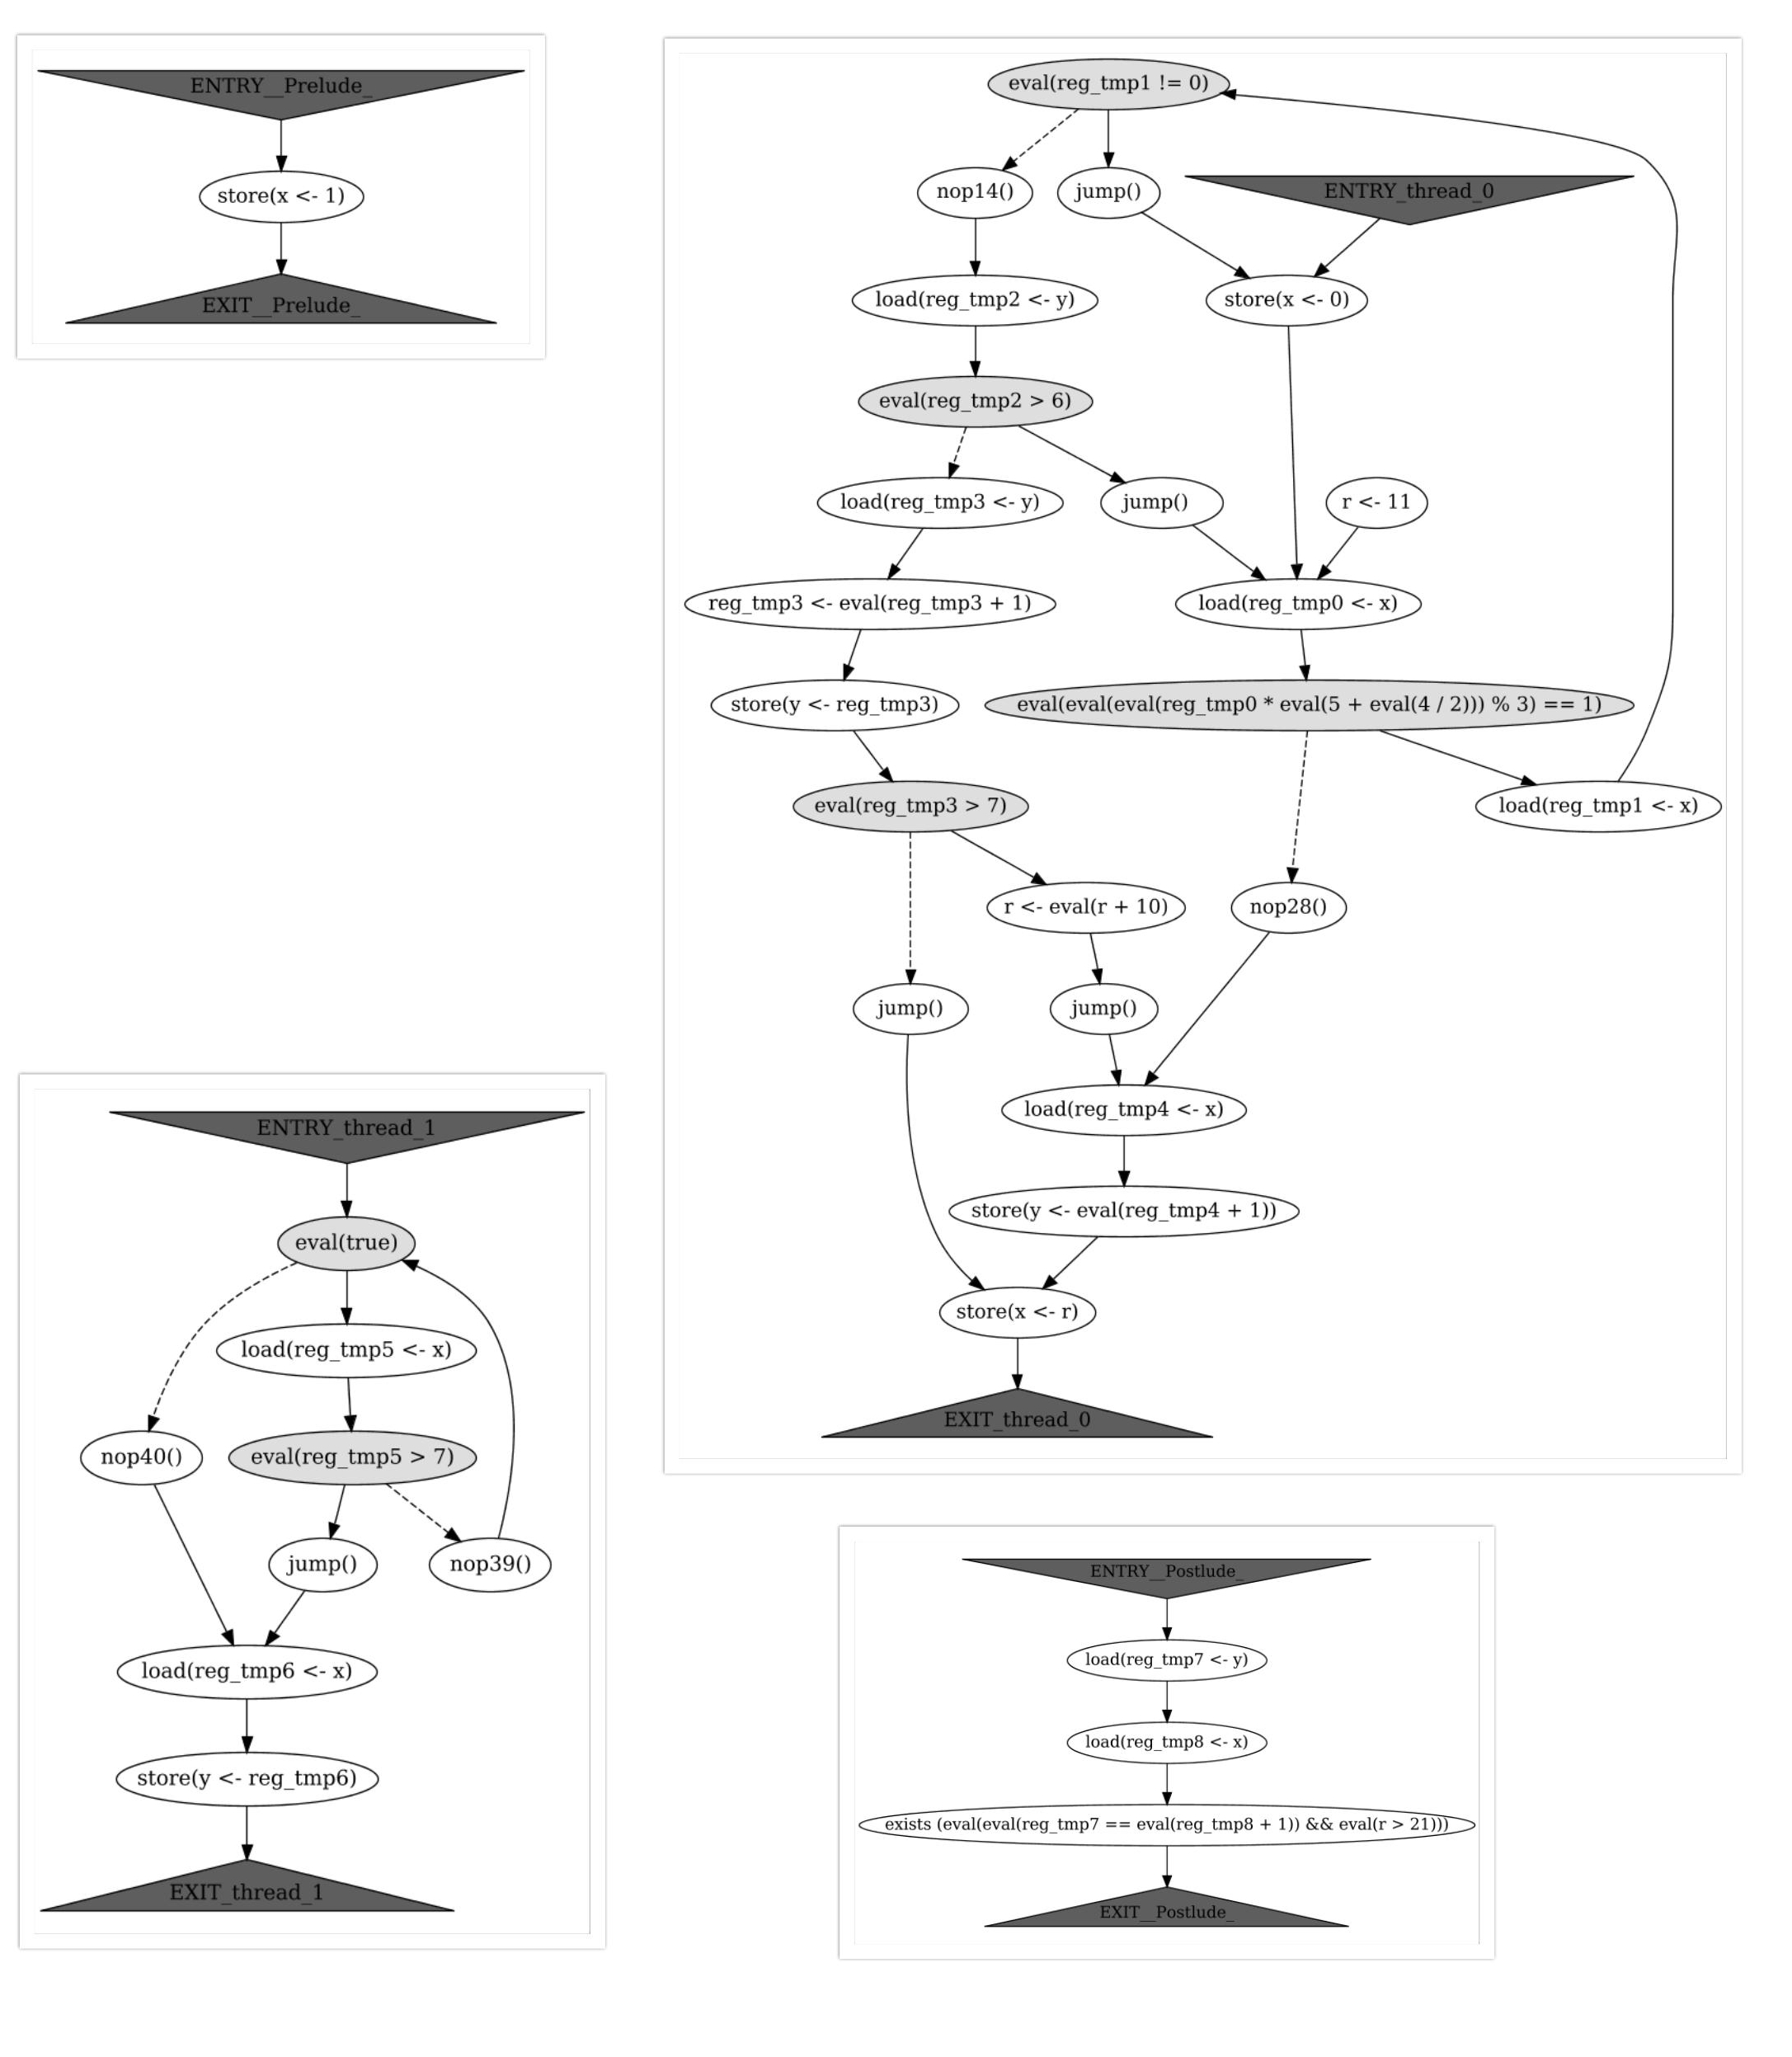
\includegraphics[width=\textwidth,keepaspectratio]{img/my/graphs/cfg-arbitrary/collage.jpg}
\caption{Control-flow components of the event-flow graphs for the code in Figure~\ref{ex:cfg-arbitrary}}
\label{ex:cfg-arbitrary:pic}
\end{figure}


\subsection{Extensible compiler mapping}

\begin{figure}%[t]
\centering
\begin{minipage}[t]{.49\textwidth}%for preventing overfull
\begin{lstlisting}
{ int x = 0; int y = 0;}

P0(volatile int* y, volatile int* x) {
  int r0;
  WRITE_ONCE(*x,1);
  r0 = READ_ONCE(*y);
}

P1(volatile int* y, volatile int* x) {
  int r0;
  WRITE_ONCE(*y,1);
  r0 = READ_ONCE(*x);
}

exists(x == 0 && y == 0)
\end{lstlisting}
\end{minipage}
\caption{SB litmus test for the Linux kernel memory model}
\label{ex:sb:kernel}
\end{figure}

%The revised design of \porthos{} tool includes the following new features:
Apart from redesigning the tool architecture and extending the input language, we added support for basic constructions used in \textit{Kernel litmus tests}~\cite{alglave2018frightening}.
Although, current version of \porthos[2] only supports some basic macros of the Linux kernel (such as \lstinline{READ_ONCE} and \lstinline{WRITE_ONCE} for atomic load and store with relaxed memory ordering) as the support for kernel-specific memory barriers goes out of the scope of current thesis.
Note that, comparing to the \porthos[1], adding support for new functions in \porthos[2] does not require changing the input language grammar, this is carried by invocation hooking mechanism described in Section~\ref{ch:impl:proc:x-compiler}.

As an example, consider the Store Buffering litmus test for the Linux kernel in Figure~\ref{ex:sb:kernel} (which is similar to the one presented in Figure~\ref{simple_wmm_x86}).
When verifying this litmus test by \porthos[2] in the state reachability mode, the test passes for TSO memory model and fails for SC model.

